\documentclass[12pt]{article}

% Prevent words to overflow over the margin
% \sloppy  % Alternative command
\emergencystretch 3em

% Math
% the journal version already loads these packages
\usepackage{amsmath,amssymb,amsthm}
\renewcommand{\qedsymbol}{$\blacksquare$}

% Images and plots
\usepackage{subfig}
\usepackage{verbatim}
\usepackage{graphicx}
\graphicspath{ {images/} }
\usepackage{pgfplots}

\usepackage{mathtools}
\usepackage{enumitem}
\usepackage{multirow}
\usepackage{algorithm}% http://ctan.org/pkg/algorithms
\usepackage[noend]{algpseudocode} % Avoid "end" and make it look cleaner

\usepackage[margin=1in]{geometry}
% Tables
\usepackage{csvsimple}	% reading CSV files in tables
\usepackage{booktabs}   % Nicer Tables
\usepackage{adjustbox}  % To adjust table length
\usepackage{appendix}
\usepackage{multicol}
\usepackage{algorithm}
\usepackage{algpseudocode}
% Hyper-references
\usepackage{hyperref}
\usepackage[nottoc]{tocbibind}

% Acronyms
\usepackage[xindy, acronyms]{glossaries}   % Glossaries and Acronyms
\makeglossaries

% Other 
\usepackage[textsize=tiny, color=blue!20]{todonotes}
\newcommand{\AAANote}[1]{\todo[inline, caption={}]{ Amirali: #1}}
\newcommand{\ColeNote}[1]{\todo[inline, caption={}]{ Cole: #1}}
\newcommand{\priv}{\text{IPT}}
\newcommand{\privuip}{\text{IPT}^\text{IP}}
\newcommand{\privlip}{\text{IPT}_\text{IP}}
\newcommand{\privsdp}{\text{IPT}^\text{SDP}}

% Definitions
% Stochastic optimization
\newcommand{\uncset}{{\mathcal{U}}}
\newcommand{\uMat}{\texttt{\textbackslash uMat}}

% Commands
\newcommand{\eg}{{\it e.g.}}
\newcommand{\ie}{{\it i.e.}}

% Sets
\newcommand{\ones}{\mathbf 1}
\newcommand{\reals}{{\mbox{\bf R}}}
\newcommand{\integers}{{\mbox{\bf Z}}}
\newcommand{\symm}{{\mbox{\bf S}}}  % symmetric matrices
\newcommand{\NPhard}{\mbox{$\mathcal{NP}$-hard}}  % symmetric matrices
\newcommand{\prob}{{\mathbf P}}
\newcommand{\distrib}{{\mathcal P}}
\newcommand{\identity}{I}
\newcommand{\tpose}{T}
\newcommand{\nullspace}{{\mathcal N}}
\newcommand{\range}{{\mathcal R}}
\newcommand{\Rank}{\mathop{\bf Rank}}
\newcommand{\Tr}{\mathop{\bf tr}}
\newcommand{\diag}{\mathop{\bf diag}}
\newcommand{\lambdamax}{{\lambda_{\rm max}}}
\newcommand{\lambdamin}{\lambda_{\rm min}}
\newcommand{\Expect}{{\mbox{\bf E}}}
\newcommand{\Co}{{\mathop {\bf Co}}} % convex hull
\newcommand{\dist}{\mathop{\bf dist{}}}
\newcommand{\epi}{\mathop{\bf epi}} % epigraph
\newcommand{\Vol}{\mathop{\bf vol}}
\newcommand{\dom}{\mathop{\bf dom}} % domain
\newcommand{\intr}{\mathop{\bf int}}
\newcommand{\dif}{\text{d}}
\newcommand{\sign}{\mathop{\bf sign}}
\newcommand{\round}{\mathop{\bf round}}
% \newcommand{\define}{\coloneqq}
\newcommand{\define}{=}
\newcommand{\defn}{\define}
\newcommand{\norm}[1]{\| #1 \|}
\renewcommand{\Re}{\reals}
\newcommand{\set}[2]{\{ #1 \mid #2 \}}

% Already defined commands in journal version

% Create theorems and other environments
\newtheorem{theorem}{Theorem}[section]  % Restart counter every section
\newtheorem{lemma}{Lemma}[section]  % Restart counter every section
\newtheorem{corollary}{Corollary}[theorem]  % Restart counter every theorem
\newtheorem{proposition}{Proposition}[section]
\newtheorem{assumption}{Assumption}[section]
\newtheorem{definition}{Definition}[section]
\newtheorem{example}{Example}[section]
\newtheorem{exercise}{Exercise}[section]
\newtheorem{remark}{Remark}[section]
\newtheorem{problem}{Problem}[section]



% Trees
\newcommand{\tree}{\mathcal{T}}

% Other
\newcommand{\tb}{\textbf}
\newcommand{\mr}{\mathbb{R}}
\newcommand{\mc}{\mathcal}
\newcommand{\sbs}{\subseteq}
\newcommand{\sps}{\supseteq}
\newcommand{\prf}{\textbf{\underline{Proof:}} }
\newcommand{\ans}{\textbf{\underline{Answer:}} }
\newcommand{\lma}{\textbf{\underline{Lemma:}} }

% Acronyms
\newacronym{IPT}{IPT}{Information Privacy Tradeoff Problem}
\newacronym{GIPT}{GIPT}{Generalized Information Privacy Tradeoff Problem}
\newacronym{KNAP}{KNAP}{Knapsack Problem}
\newacronym{MIP}{MIP}{Mixed Integer Program}
\newacronym{SOCP}{SOCP}{Second Order Cone Program}
\newacronym{LP}{LP}{Linear Program}
\newacronym{IP}{IP}{Integer Program}
\newacronym{poi}{poi}{Person of Interest}


% Bibliography
\bibliographystyle{acm}




\begin{document}



\title{Information Privacy Tradeoff}
\author{Cole Becker, advised by Amir Ali Ahmadi}
\date{ORF 375 Report}
\maketitle
\section{Introduction}
An important public policy issue that has arisen in recent years is the extent to which online advertisers should be allowed to mine and sell consumers’ personal information to improve message targeting and sales. Whether it be social network platforms like Instagram and Facebook collecting personal information, or websites tracking “cookies,'' surveillance advertising has intrusively commodified our personal information for the purpose of private profit. The question of how to balance personal privacy protection and information gain is not well regulated, studied, or formulated. What is a “reasonable amount” of information a company should be able to extract about a consumer, and what kinds of personal data should consumers have a justifiable expectation of keeping private? Though often debated, clear metrics and standards don’t yet exist. We introduce one possibility for defining and regulating privacy in a data-purchasing transaction, in the form of a decision problem we call \gls{IPT}. Simply put, \gls{IPT} quantifies privacy (or lackthereof) of a data purchase in terms of the degree to which revealed user data can be used to uniquely identify the user from a dataset with other users. \gls{IPT} then seeks to balance the amount of information that is gained by a data purchaser with the amount of privacy the user experiences. In this work we introduce \gls{IPT}, analyze some of its properties including computational complexity and solvability, and provide various problem bounds.

\section{Related Works}
\subsection{Differential Privacy}
Differential Privacy \cite{dwork2008differential}\cite{hassan2019differential}\cite{zhao2022survey}\cite{ji2014differential} is a relatively young field of privacy-preserving data analysis which broadly seeks to learn statistical information about a dataset without compromising the privacy of individuals. In particular, Differential Privacy is interested in quantifying (and reducing) how much the addition or removal of a user in a database will alter distributional information for the database, the assumption being is that distributional information can be shared. While related, our problem \gls{IPT} takes a slightly different approach of seeking to quantify privacy of information sharing transaction for a single user in the database. For more detailed information on differential privacy, see any of the previously referenced survey papers.

\subsection{The Knapsack Problem}
The \gls{KNAP} \cite{KelPfePis04} \cite{salkin1975knapsack} is a famous decision problem in combinatorial optimization, which seeks to determine the most valuable items to include in a knapsack from a given subset, constrained by a fixed capacity of the knapsack. While a different problem to \gls{IPT}, various complexity and algorithmic results from \gls{KNAP} can be leveraged to find similar results in \gls{IPT}.



\subsection{Submodular Maximization}
Consider a function $f:2^E \to \mr$ mapping from the power set of some ground set $S$ to $\mr$. We say that $f$ is submodular if $f(S + e) - f(S) \geq f(T+ e)-f(T)$ for any fixed subsets $S \sbs T \sbs E$. Submodular maximization \cite{krause2014submodular}\cite{mccormick2005submodular} problems occur when seek a maximizing subset $A \sbs E$ for a submodular function $f$. While not yet well understood, there may be some relevant results from the submodular maximization literature to improve or inform \gls{IPT} algorithms.   

\subsection{L0 Norm formulations}
The formulation we discover for \gls{IPT} contains the L0 pseudonorm, which counts the number of non-zero entries in a vector. While the L0 norm is not a true norm, and thus creates a non-convex inequality constraint, various works \cite{Alper} \cite{feng2013complementarity}, exist which produce closely related convex, or integer constraint reformulation of the L0 norm. Investigating these results could prove useful for future work with \gls{IPT}.


\section{The Problem}
We consider the following decision problem, we denote \gls{IPT}
\paragraph{Input:}
Consider a dataset $\mc{D} = \{d_i\}_{i\leq m} \sbs \mr^n$ where $d_i \in \{0,1\}^n$, and denote $D\in \mr^{m\times n}$ as the matrix containing this data. We can imagine for example that $m$ is the number of people in the dataset, and $d_i\in \mr^n$ represents a binary feature vector of information on $n$ features for the $i$th person. In addition, you are given a non-negative weight vector $w\in \mr^n$ representing the relative importance of each the $n$ features, some number $r \in [0,1]$ and an index $k \in \{1,...,m\}$. Finally we also take in a non-negative number $l \in \mr$. 
\paragraph{Question:}
Is there a way to select a subset of features of $d_k$, indexed by $x\in \{0,1\}^n$ such that $w^T x \geq l$ and the subset features of $d_k$ are shared by at least $rm$ people in the dataset ($d_k$ included). \tb{Note}: Throughout the entirety of this paper, we will assume $k = 0$ unless otherwise specified, and we will refer to $d_k$ as \gls{poi}.
\subsection{Motivation}
Suppose you are a company holding such a dataset $\mc{D}$ containing various boolean features of a large quantity of individuals. Some advertising company Ad.co comes to you, and wants to purchase the data of some individual $k$ to run some targeted advertising of their own. In order to convey which features they are most interested in knowing, or which features are most useful to their advertising campaign, they supply you with a weight vector $w$ which represents how much Ad.co values knowing each feature of individual $k$ in your dataset. However, as your company must comply with privacy regulations, you are not allowed to share too much information about individual $k$ which would distinguish them too much. Specifically, the features you reveal to Ad.co about individual $k$ must also be shared by $100 * r\%$ of the members of your dataset. Your task is to maximize the useful information you can share with Ad.co while satisfying the imposed privacy constraints.


\subsection{Formulation of \gls{IPT}}
Taking all the same inputs from the above problem, let us first define a helper matrix $K \in \mr^{m\times n}$ as
\begin{align*}
    K_{ij} = \begin{cases}
        0 & \text{ if } D_{ij} = D_{kj} = (d_k)_j\\
        1 & \text{ otherwise}
    \end{cases}
\end{align*} 
We note that \gls{IPT} can be reduced to the following non-convex optimization problem
\begin{equation}
	\label{eq:priv} 
    \tag{$\priv$} 
	\begin{array}{lll}
		\priv = & \underset{x}{\text{maximize}} & w^T x \\
		& \mbox{subject to} & ||K x||_{0}  \leq C \\
        && x_i \in \{0,1\}
		\end{array}
\end{equation}
where here for ease of notation we define $C: = \lceil m(1-r)\rceil$ and the answer to the decision question is given by whether $\priv \geq l$. To see why the constraint in this problem is equivalent to the requirement that the subset $x$ of $d_k$'s features is shared by at least $rm$ people, note that  \[(Kx)_i = \begin{cases}
    0 & \text{ if } d_i \text{ shares the same } x \text{ features with } d_k \\
    > 0 & \text{ otherwise}
\end{cases}
\]
so the number of 0-elements in $Kx$ must be greater than $mr$ or equivalently, the number of non-zero elements must be less than $m(1-r)$. For ease of notation, we will use $C = \lceil m(1-r)\rceil$ for the rest of the paper.
\subsection{Graph Interpretation}
Another way to interpret this problem is via a graph optimization problem. Given a $K$ matrix, we can define a respective bipartite graph $G(P,F,E)$ with vertex subsets $P,F$ representing the people (excluding \gls{poi}) in our dataset, and the features we know of. Two vertices $p$ and $f$ share an edge if person $p$ is unique from \gls{poi} in feature $f$. An example $K$ matrix and bipartie graph is pictured below
\begin{figure}[H]
    \centering
    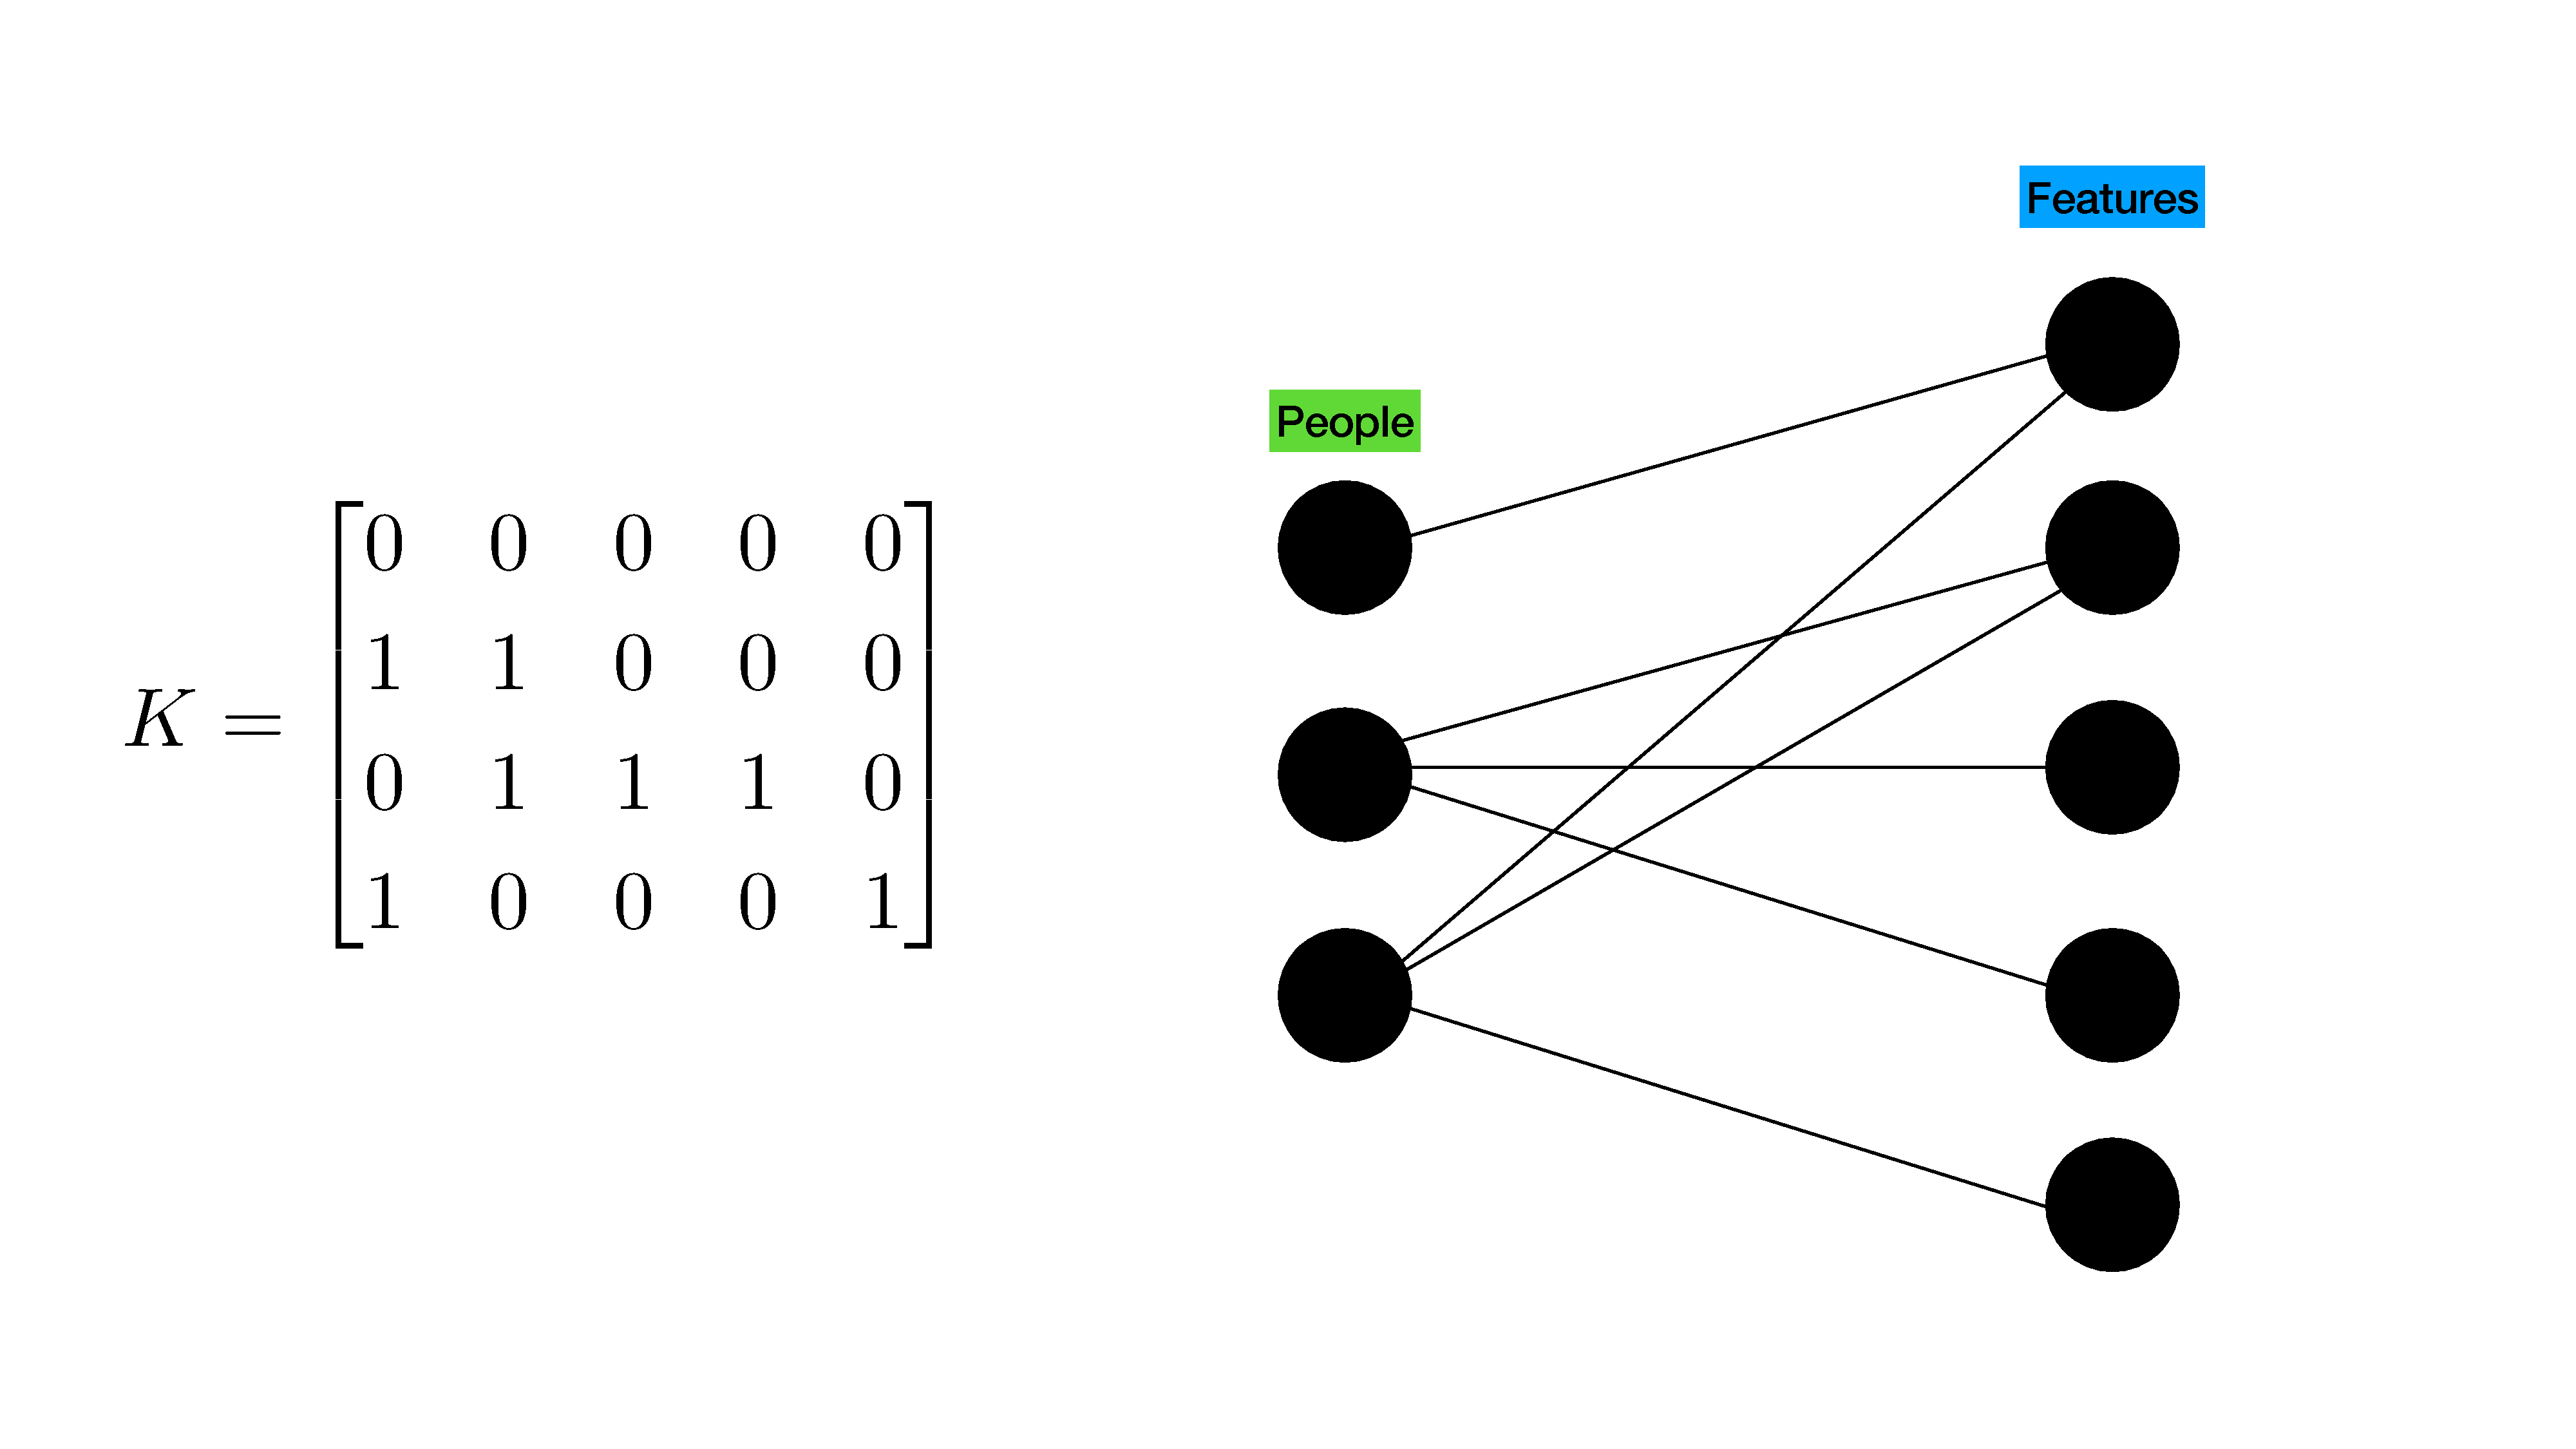
\includegraphics[width = 14cm]{../images/graph_ipt.pdf}
    \label{fig:graph}
\end{figure}
Given this Interpretation, we can define the following equivalent optimization problem:
\begin{equation}
	\label{eq:priv_graph} 
    \tag{$\priv$} 
	\begin{array}{lll}
		\priv = & \underset{X \sbs V(F)}{\text{maximize}} & w^T X \\
		& \mbox{subject to} & |N(X)| \leq C \\
		\end{array}
\end{equation}
where $N(X)$ represents the vertex subset of all the neighbors of $X$. Here we note that for each $x\in X$, $N(x)$ represents all the individuals with feature $x$ distinct, so we have that $|N(X)|$ really is equivalent of $||K X||_0$ from the original formulation.
\subsection{Related Problem}
A closely related problem is the following problem is \gls{GIPT}
\[\text{GIPT} = \text{argmin}_k \ \priv_k\]
where $\priv_k$ represents the information privacy tradeoff of the $k$th individual in the dataset. We can think of the minimum over all such individauls as the most distinguishable/unique, or least anonymous individual. This is the individual for whom you can reveal the least information before they begin to be distinguishable from $r$\% of the dataset. 
In a closely related problem, we have 
\[\text{argmax}_k \ \priv_k\]
which can be thought of as the most anonymous and least unique individual in the dataset. 
\paragraph{20 Questions}
A simple way to think of this problem is as a game. Given a dataset of possible things to guess in a game of twenty questions (or people to learn information from), you would like to choose the least distinguishable individual to maximize the amount of guesses. \tb{However}, it is important to note that $\text{argmax}_k \ \priv_k$ isn't exactly identical to 20 questions. We might ask ourself what is the goal of twenty questions? The goal as a guesser is to reveal the features that on average leave the fewest members remaining. Here we are interested in privacy, so it would be more of a word producing game. We would want to produce a word such that on average, it is very anonymous. In other words, no matter what features you reveal, it doesn't narrow down your search very much. $\text{argmax}_k \ \priv_k$, means that you can reveal lots of features without narrowing the search down much. However think of the worst case scenario, in which there is one feature that such an individual has that she shares with nobody. This would make them distinguishable in a way, even if they were very anonymous with respect to their other features. So perhaps it isn't entirely obvious that $\text{argmax}_k \ \priv_k$ is the best metric for a 20 questions guessing game.

\section{Complexity of \gls{IPT}}
\begin{theorem}
    \gls{IPT} is NP-complete
\end{theorem}
\begin{proof}
    It is sufficient to show that \gls{IPT} $\in $ NP and that \gls{KNAP} $ \longrightarrow$  \gls{IPT}
    \begin{enumerate}
        \item \gls{IPT} $\in $ NP: Given a certificate solution $x^*$ to $\priv$, it is easy to check that the constraints are satisfied, and that $w^T x^* \geq l$
        \item \gls{KNAP} $ \longrightarrow$  \gls{IPT}: Consider the classic \gls{KNAP}:
        \\ \tb{Input:}
        \textit{$w \in \mr^n$ a weight vector of $n$ items, $p \in \mr^n$ a price vector for the items, $W\in \mr$ a weight capacity, and $P \in \mr$}
        \\ \tb{Question:}
        \textit{Is there a set of items of combined weight less than $W$ but with combined price greater than $P$?}
        \\~\\ 
        Using these inputs we will construct an instance of \gls{IPT} (Note we will assume for convenience that $W \in [0,1^Tw]$. If not we can define a new $W$ that is respective endpoint). To begin, set $m = 1+ 1^Tw$ and construct the following data matrix $D \in \mr^{m\times n}$ by the following procedure:
        \begin{enumerate}
            \item Set the first row of $D$ to a row of all $0$s
            \item For each weight $w_i$, $i\in\{1,...,n\}$ add $w_i$ copies of the one hot encoded row vector $e_i$. As an example:
            \[w = [3,1,2,1] \implies D = \begin{bmatrix}
                0&0&0&0 \\
                1&0&0&0 \\
                1&0&0&0 \\
                1&0&0&0 \\
                0&1&0&0 \\
                0&0&1&0 \\
                0&0&1&0 \\
                0&0&0&1 
            \end{bmatrix}\]
            This is the data matrix $D$ we will consider. Note that the auxiliary matrix $K$ used in \gls{IPT} is identical to $D$ via the way we constructed it.
        \end{enumerate}
        In addition, set $r = 1 - W/m$ (whereby assumption on $W$ we have $r \in [0,1]$), $l = P$, $k = 1$ the first row, and $\bar{w} = p$, the information weighting vector. We now have an instance of \gls{IPT}. In terms of the \gls{KNAP} variables, the equivalent \gls{IPT} problem looks like the following:
        \begin{equation}
            \begin{array}{lll}
                \priv(\text{KNAP}) = & \underset{x}{\text{maximize}} & p^T x \\
                & \mbox{subject to} & ||D x||_{0}  \leq W \\
                && x_i \in \{0,1\}
                \end{array}
        \end{equation}
        Notice the problem construction requires a polynomial amount of operations, as the size of $D = n * (1+ 1^T w)$, and everything else requires an affine amount of operations.
        We would now like to show the following equivalence between the problems. 
        \[\text{\gls{KNAP}} \geq P \iff \text{IPT(KNAP)} \geq P\]
       (\underline{$\Longrightarrow$}): Consider a solution $\hat{x}\in \{0,1\}^n$ to \gls{KNAP} satisfying the weight constraints and with $p^Tx \geq P$. This same solution $\hat{x}$ will be feasible to IPT(KNAP). To see why, just note that $||Dx||_0 = w^Tx$ is equivalent to taking the sum of the weights, because the construction of $D$ and $x$ mean that $||Dx||_0 = 1^TDx$ and $1^TD = w$ by construction. \\
       (\underline{$\Longleftarrow$}): The backwards argument is similar, but we need to build back the weight vector $w$ from the matrix $D$. To do so we again note that $w = 1^TD$, and then the problem is identical to knapsack.
    \end{enumerate}
\end{proof}


\section{Bounds and Relaxations for \gls{IPT}}
\subsection{\gls{MIP} Bounds}
As written in its L-0 form, \gls{IPT} is not even a mixed-integer program. Here we investigate affine relaxations of the L-0 norm and possible interpretations.
\subsubsection{\gls{MIP} Upper Bound}
We write an IP relaxation of \gls{IPT} as the following problem
\begin{equation}
	\label{eq:privuip} 
    \tag{$\privuip$} 
	\begin{array}{lll}
		\privuip = & \underset{x\in\mr^n}{\text{maximize}} & w^T x \\
		& \mbox{subject to} & \mathbf{1}^TKx \leq m(1-r)\mathbf{1}^Tx \\
        && x_i \in \{0,1\}
		\end{array}
\end{equation}
Where we have $\priv \leq \privuip$. To see why we would like to show
\[x \text{ feasible to } \priv \implies x \text{ feasible to } \privuip.\]
Consider $x^*$ feasible to $\priv$. If $x^* =0$ then $x^*$ is clearly feasible to $\privuip$ as both constraints are trivially satisfied. Now suppose $x^*\neq 0$, we want to show that \[\frac{\mathbf{1}^TKx^*}{\mathbf{1}^Tx^*} \leq C,\] or equivalently, that $\frac{\mathbf{1}^TKx^*}{\mathbf{1}^Tx^*} \leq ||Kx^*||_0$. The key is to notice is that $(Kx^*)_i \leq \mathbf{1}^Tx^*$ for all $i\leq m$ due to the binary nature of the entries of $K$ and $x^*$, which means that 
\[\left(\frac{\mathbf{1}^TKx^*}{\mathbf{1}^Tx^*}\right)_i = 
\begin{cases}
    0 & \text{ if } (Kx^*)_i = 0 \\
    \leq 1 & \text{ otherwise}
\end{cases}
\]
from the above statement we have
\[\frac{\mathbf{1}^TKx^*}{\mathbf{1}^Tx^*} \leq ||Kx^*||_0\]
so $x^*$ is feasible to $\privuip$, and $\priv \leq \privuip$.
% and consider an indicator vector $y \in \mr^m$ with 
% \[y_i = \begin{cases}
%      1 & \text{ if } d_i \text{ shares the same } x \text{ features with } d_k \\
%     0 & \text{ otherwise.}
% \end{cases}
% \]
%  We want to ensure that $1^T y \geq rm$. However we claim that $\frac{1^T \bar{K}x}{1^Tx} \geq 1^T y$. To see why, note that $(\bar{K}x)_i$ counts the number of features out of $x$ that $d_i$ and $d_k$ share, so 
% \[\left(\frac{\bar{K}x}{1^T x}\right)_i = 
% \begin{cases}
%     1 & \text{ if } d_i \text{ shares the same } x \text{ features with } d_k \\
%     \in [0,1) & \text{ otherwise}
% \end{cases}\]
% Of course to be sure that at least $rm$ individuals share the same features as the $d_k$th individual, we can sum to get $\frac{1^T\bar{K}x}{1^T x} \geq 1^Ty \geq rm$, and we get the constraint in $\privl$. 


\subsubsection{\gls{MIP} lower bound}
Next consider the following linear integer program
\begin{equation}
	\label{eq:privlip} 
    \tag{$\privlip$} 
	\begin{array}{lll}
		\privlip & = \underset{x}{\text{maximize}} & w^T x \\
		&\mbox{subject to} & \mathbf{1}^TKx \leq C \\
        && x_i\in \{0,1\}
		\end{array}
\end{equation}
To see why $\privlip \leq \priv$, we would like to show that 
\[x \text{ feasible to } \privlip \implies x \text{ feasible to } \priv.\]
Fix $x^*$ feasible to $\privlip$. Due to binary nature of $K$ and $x^*$, we know $Kx^*$ is a non-negative integer vector. This means $\mathbf{1}^TKx^* = ||Kx^*||_1$ and so we have \[ ||Kx^*||_0 \leq ||Kx^*||_1 = \mathbf{1}^T K x^* \leq C\]
so $x^*$ is feasible to $\priv$, and $\privlip \leq \priv$

\subsubsection{Relation to \gls{KNAP}}
Succinctly, we have shown that \ref{eq:privlip} $\leq$ \ref{eq:priv} $\leq$ \ref{eq:privuip} due to the fact that for non-zero $x$, we have \[\frac{\mathbf{1}^TKx}{\mathbf{1}^Tx} \leq ||Kx||_0 \leq \mathbf{1}^TKx\]
However if we define $\alpha := \mathbf{1}^TK$, then we can interpret \ref{eq:privlip} as a knapsack problem, where each item in the knapsack corresponds to a feature in our dataset. In this way, we can interpret the $i$th item $\alpha_i$ as a collection of people with feature $i$ distinct from our choice user. In other words, the weight of each item $\alpha_i$ is the number of people with feature $i$ distinct. This means that for a chosen subset of items (or features) $x$ to put in our knapsack, we can interpret the total weight of each of these items $\alpha^T x = \mathbf{1}^TKx$, as the total number of people in our knapsack, where we count each person once for each distinct feature they have. This means if person $i$ has 4 distinct features from \gls{poi}, then they will be counted 4 times and provide a weight of 4 into the knapsack. As $(Kx)_i$ represents the number of unique features individual $i$ has from \gls{poi}, every person is added $(Kx)_i$ times to the bag. In other words, $(Kx)_i$ represents how many items individual $i$ is in out of the subset $x$. In this way, counting the number of "unique" people in our knapsack corresponds to counting the number of people with $\geq 1$ distinct feature from \gls{poi}, which is equivalent to $||Kx||_0$. To illustrate this, consider an example $K$, and feature vector $x$ 
\[K = \begin{bmatrix}
    0&0&0 \\
    1&0&0 \\
    1&1&0\\
    0&1&1
\end{bmatrix}, \quad x = [1,1,0]^T, \quad Kx = \begin{bmatrix}
    0\\1\\2\\1
\end{bmatrix}, \quad \alpha = \begin{bmatrix}
    2&2&1
\end{bmatrix}\]
Where we he have three individuals (call them A,B,C) aside from \gls{poi} (row 1) and three features. We can view the items in our knapsack $\alpha = \mathbf{1}^TK$ as the following objects (one for each of the three features).
\begin{figure}[H]
    \centering
    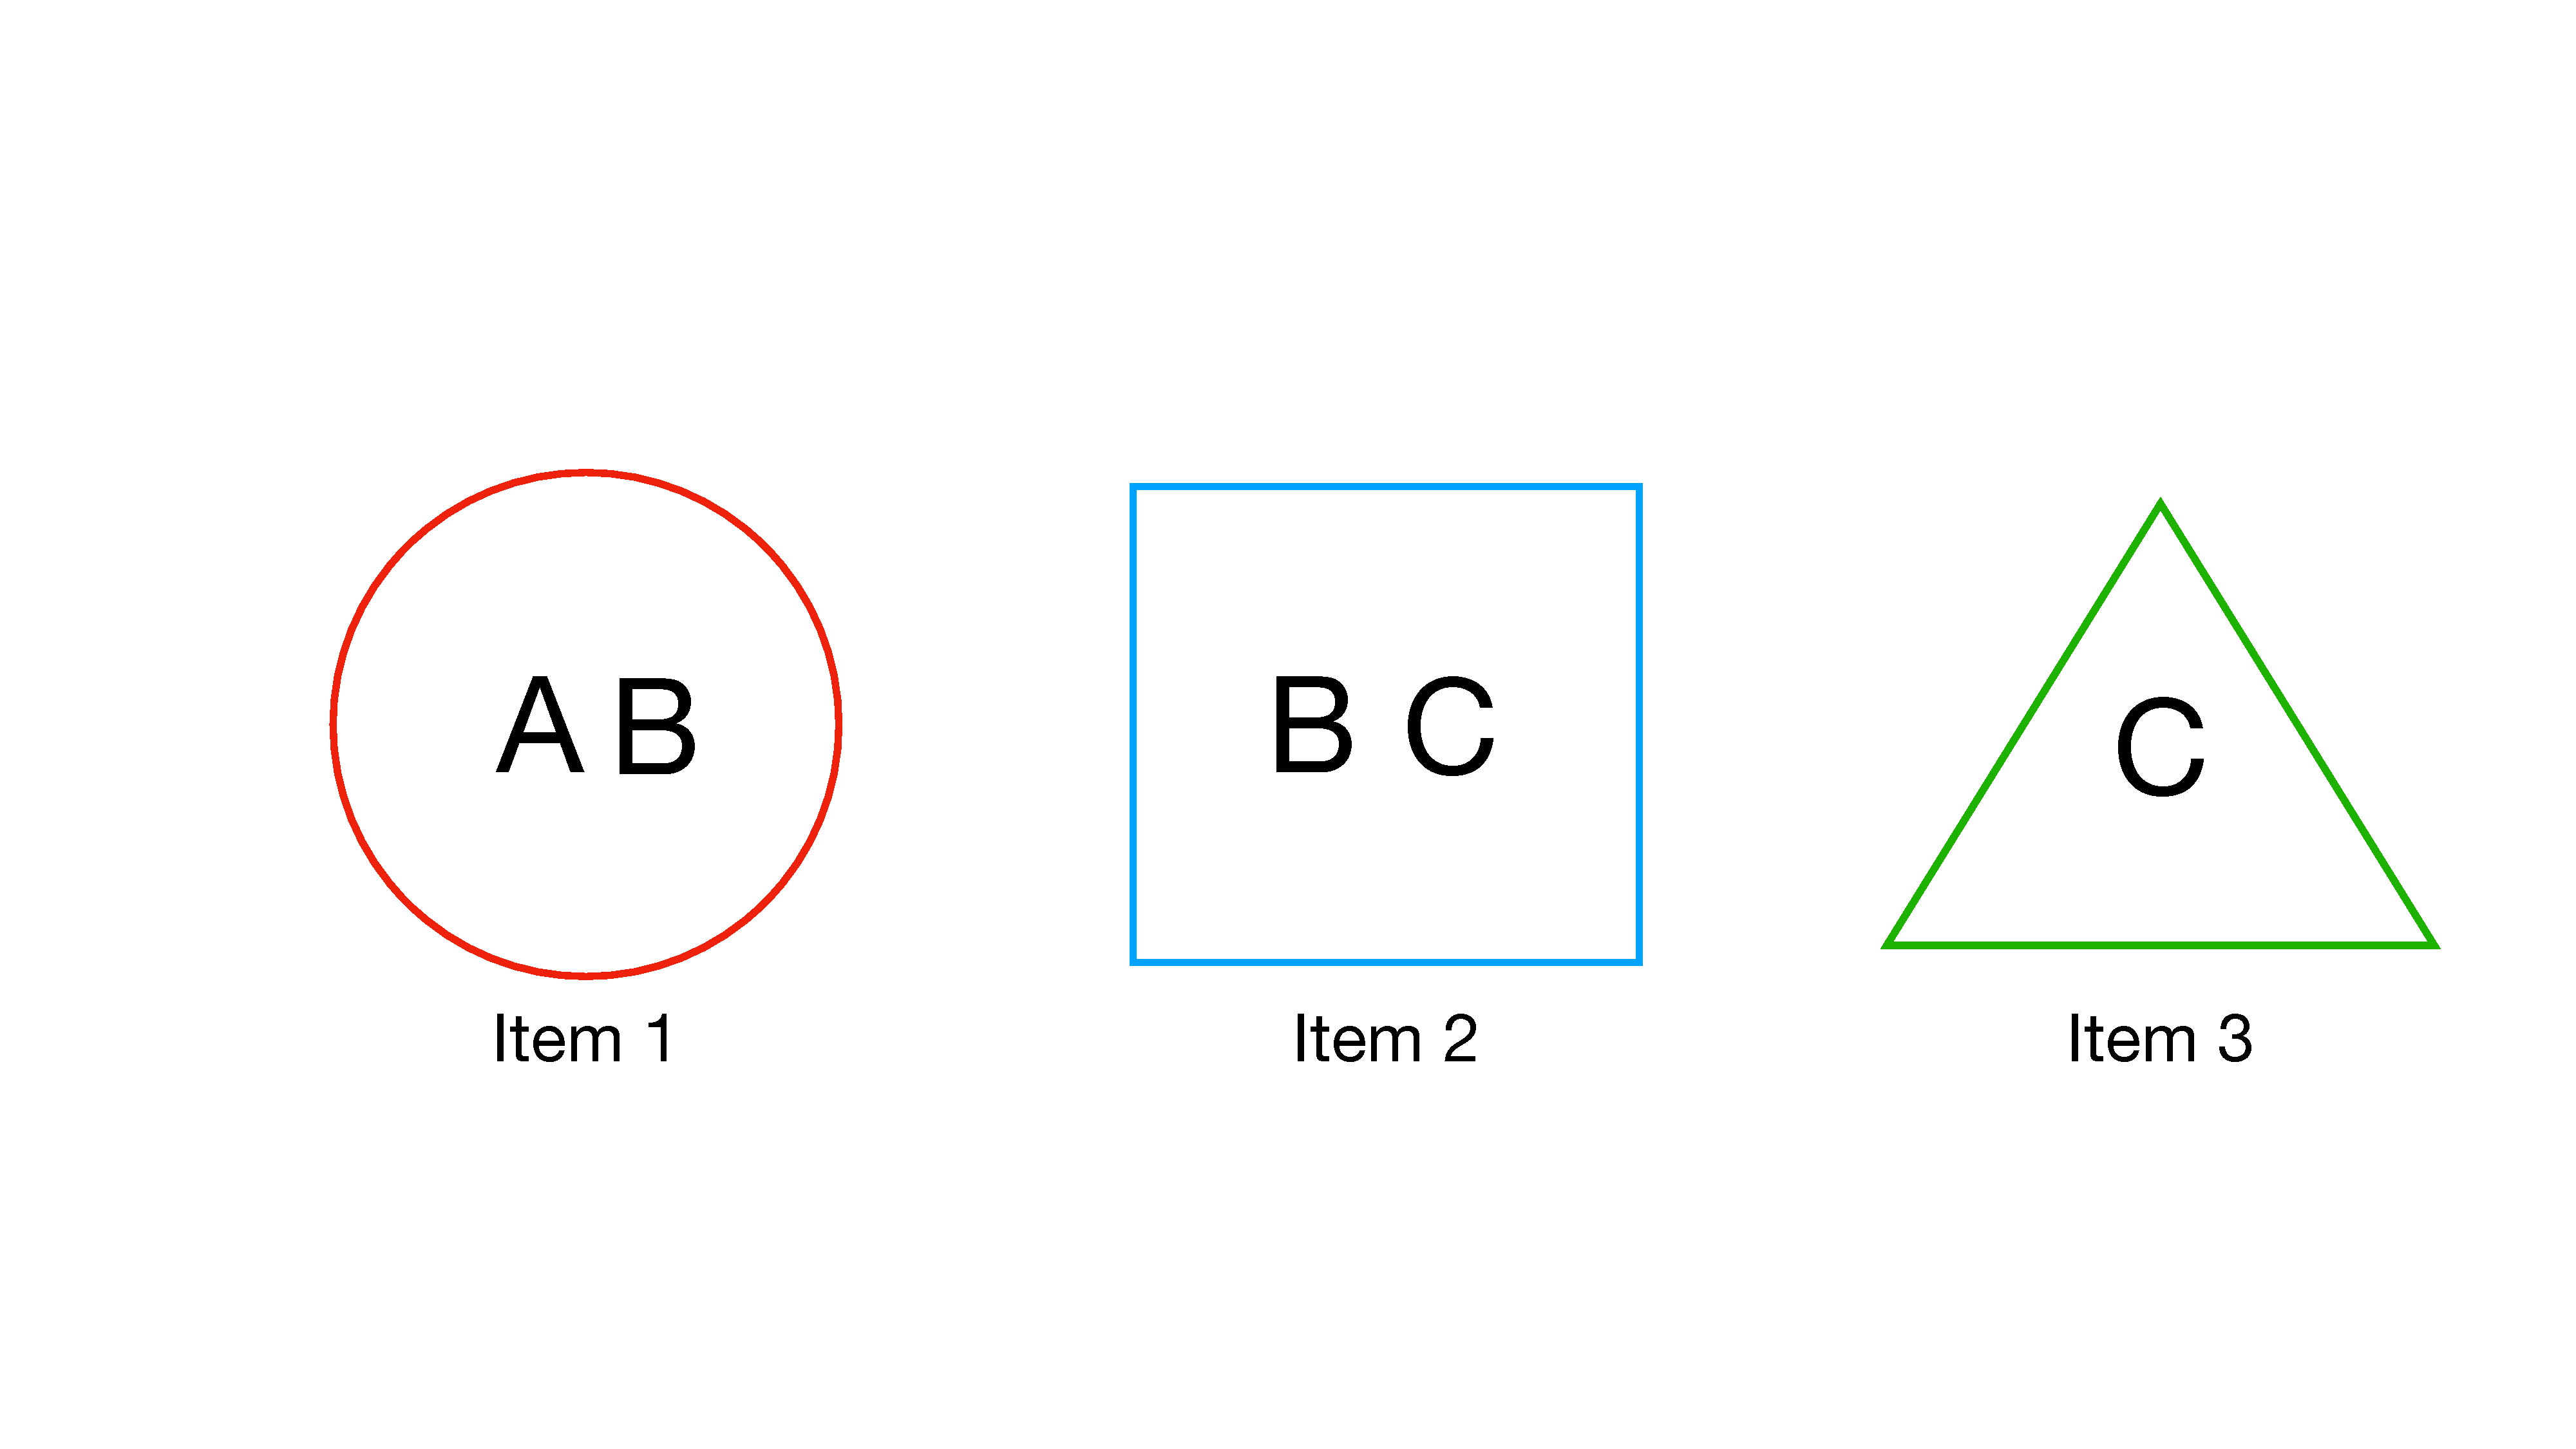
\includegraphics[width = 14cm]{../images/knap_intuition.pdf}
    \label{fig:items}
\end{figure}
Here we only select the first two items $x = [1,1,0]^T$, so the weight of our knapsack $\mathbf{1}^TKx = \alpha^Tx = 4$. However, there are only three unique individuals in our knapsack, as we double count $B$. In order to only count $B$ once, we just take $||Kx||_0 = 3$ (i.e. count the number of non-zeros)
% The process of removing the duplicates, is equivalent to taking
% \[Kx = \begin{bmatrix}
%     0 \\1 \\2\\1
% \end{bmatrix} \to \begin{bmatrix}
%     0 \\1 \\1 \\1
% \end{bmatrix}\]
% To summarize we have 
% \begin{align*}
%     (Kx)_i &= \text{ number of distinct features of person $i$ from subset $x$} \\
%     \alpha_i = (\mathbf{1}^TK)_i &= \text{ number of }
% \end{align*}

\subsection{Convex Upper Bounds}
\subsubsection{SDP Upper bound}
Consider the following SDP:
\begin{equation}
	\label{eq:privsdp} 
    \tag{$\privsdp$} 
	\begin{array}{lll}
		\privsdp = & \underset{x\in\mr^n}{\text{maximize}} & w^T x \\
		& \mbox{subject to} &  
        \begin{bmatrix}
            \begin{matrix}
                X
            \end{matrix}  & 
            \begin{matrix}
                Z
            \end{matrix} & x \\
            \begin{matrix}
                Z^T 
            \end{matrix} & 
            \begin{matrix}
                Y 
            \end{matrix} & y \\
            x^T & y^T & 1
        \end{bmatrix} \succeq 0\\
        && x_i = X_{ii}, \quad \forall i\leq n\\
        && y_j = Y_{jj}, \quad \forall j \leq m\\
        && \mathbf{1}^Ty \geq rm \\
        && 0 \leq x,y,X,Y,Z \leq 1
		\end{array}
\end{equation}
To see why $\priv \leq \privsdp$, we would like to show that
\[x^* \text{ feasible to } \priv \implies \exists x,y,X,Z,Y \text{ feasible to }\privsdp\] 
Take $x^*$ feasible to $\priv$ and let $x = x^*$. Next define a vector $y \in \mr^n$ with each entry define as
\[y_i = \begin{cases}
    1 & \text{if } (Kx)_i = 0 \\
    0 & \text{otherwise}
\end{cases}\]
In other words, $y_i = 1$ if all subfeatures of individaul $i$ are shared with \gls{poi}. As $\mathbf{1}^Ty$ represents the number of individauls indistinguishable from \gls{poi}, clearly we will satisfy the constraint that $\mathbf{1}^Ty \geq rm$ by $x$ being feasible to $\priv$. As $x,y$ are also binary vectors, we satisfy that equality as well. Next define \[X = xx^T, \ Z = xy^T, \ Y = yy^T\]
and by Schur's complement, we satisfy the psd constraint, and the equality constraints. So we have feasiblity to $\privsdp$. Note that of course we can add on a the linear constraint from the MIP upper bound $\mathbf{1}^TKx \leq C\mathbf{1}^Tx$ to get a tighter SDP relaxation.\

\section{Algorithmic approximations}
\subsection{Greedy Lower Bound}
    Define $\bar{K} = 1 - K$ as the matrix with the entries in $K$ flipped. Now for any column $\bar{K}_i$ of matrix $\bar{K}$, define its value \[v_i = (1^T \bar{K}_i) w_i\] and order the columns from largest to smallest value, then perform a greedy selection algorithm by selecting the columns with the largest value up until the privacy constraint is violated. The idea is we both want to select columns which are weighted highly and who share features with the $k$th column.  Note that we can always rewrite $\mathbf{1}^T\bar{K} = m - \mathbf{1}^TK$, so this formulation need not involve a new $\overline{K}$.\footnote{Inspired by question 1 on the 2016 ORF 363 Final}. Together, the greedy algorithm is the following:
    \begin{algorithm}
    \caption{Greedy Algorithm for \gls{IPT}}\label{alg:greedy}
    \begin{algorithmic}
        \State $v_i \gets (\mathbf{1}^T\bar{K}_i)w_i, \quad \forall i\leq n$
        \State $x_i \gets 0, \quad \forall i\leq n$
        \For{$j = 1:n$}
        \State $k = $ idx of $j$th largest element of $v$
        \State $x^{\text{copy}} \gets x$
        \State $x^{\text{copy}}_k \gets 1$
        \If{$||Kx^{\text{copy}}||_0 \leq C$}
            \State $x \gets x^{\text{copy}}$
        \EndIf
        \EndFor
        \Return $x$
        \end{algorithmic}
    \end{algorithm}
of course the output of this algorithm $x^*$ will be feasible to \gls{IPT}, and therefore $w^Tx^*$ will be a lower bound.
\subsection{\gls{KNAP} Dynamic Programming Lower Bound}
Inspired by the original Dynamic Programming Knapsack algorithm from \cite{KelPfePis04} we give a dynamic programming lower bound with a runtime complexity of $\mathbf{O}(n C)$. This works in the following way: first we define a smaller \gls{IPT} problem 
\begin{equation}
	\label{eq:priv_j} 
    \tag{$\text{IPT}_j(d)$} 
	\begin{array}{lll}
		\priv_j(d) = & \underset{x}{\text{maximize}} & \sum_{i=1}^j w_i x_i \\
		& \mbox{subject to} & ||K x||_{0}^j  \leq d \\
        && x_i \in \{0,1\}
		\end{array}
\end{equation}
where we use the notation $||y||_0^j$ to represent the number of non-zero elements in the first $j$ entries of some vector $y$. In other words, $\priv_j(d)$ represents the optimal value for subproblem consisting of the first $j$ features and capacity of $d$, where $d \in \{0,1,...,C\}$. We can represent the optimal subset of revealed features corresponding to the above problem as $X_j(d)$. Next, by letting $K_j$ be the $j$th column of the matrix $K$, we will define a quantity $z_j(d)$ as the following:
\[ z_j(d) = \begin{cases}
    z_{j-1}(d) & \text{ if } \mathbf{1}^T K_{j} > d \\
    \max\{z_{j-1}(d), z_{j-1}(d- \mathbf{1}^T K_{j}) + w_j\} & \text{ otherwise}
\end{cases}
\]
for $j \in \{0,...,n\}, \ d \in \{0,...C\}$, and where $z_0(d) = 0, \forall d \leq C$. The idea is that for each incremental feature $j$ we are considering. We choose to reveal $j$ only if  
\begin{theorem}
    $z_j(d) \leq \priv_j(d), \ \forall j,d$
\end{theorem}
\begin{proof}
    We will prove this by induction for any arbitrary $d$. As a base case when $j = 0$ we have $z_j(d) =\priv_j(d)$ and so the inequality is trivially satisfied. Now fixing $j$ we may assume by our inductive hypothesis that $z_{j-1}(d) \leq \priv_{j-1}(d)$. Now if $\mathbf{1}^TK_j > d$, then we get that $z_{j}(d) = z_{j-1}(d)$ and $\priv_{j}(d) = \priv_{j-1}(d)$, so the inequality is satisfied. Now consider the case where $\mathbf{1}^TK_j \leq d$. We have 
    \begin{align*}
        \max\{z_{j-1}(d), z_{j-1}(d- \mathbf{1}^T K_{j}) + w_j\} &\leq \max\{\priv_{j-1}(d), \priv_{j-1}(d- \mathbf{1}^T K_{j}) + w_j\}.
    \end{align*}
    Next recall the optimal subset $X_{j-1}(d)$ for the corresponding $\priv_j(d)$ subproblem, and define $\bar{X}_j(d) \in \{0,1\}^n$ as the optimal subset of features to reveal out of the first $j$ features, conditional on feature $j$ being revealed. By assumption let us assume $\bar{X}_j(d)$ is only defined in the case that $\mathbf{1}^T K_{j} \leq d$. In this case, denote
    \[\alpha_j := ||K \bar{X}_{j}(d)||_0 - ||K X_{j-1}(d)||_0\]
    so that $\alpha_j$ denotes the additional number of non-zero entries of (i.e. additional number of distinguishable individuals) revealing a feature $j$ would add to optimal $j-1$ subset of revealed features. By noting that \[\mathbf{1}^TK_j \geq \alpha_j\] we get that \[d - \mathbf{1}^TK_j \leq d - \alpha_j\].  Now because for any fixed $j$, $z_j(d)$ is monotonically increasing in $d$, i.e. $z_j(a) \leq z_j(b)$ for $a\leq b$, we get that $ \priv_{j-1}(d- \mathbf{1}^T K_{j}) \leq \priv_{j-1}(d- \alpha_j)$ and so we have
    \begin{align*}
        \max\{\priv_{j-1}(d), \priv_{j-1}(d- \mathbf{1}^T K_{j}) + w_j\} &\leq  \max\{\priv_{j-1}(d),\priv_{j-1}(d- \alpha_j) + w_j\} \\
        & = \priv_{j}(d)
    \end{align*}
    so we have by induction that  $z_j(d) \leq \priv_j(d), \ \forall j,d$. Solving for $z_n(C)$ will thus give us a lower bound on $\priv_n(C)$.
\end{proof}
The above lower bound on  $\priv_j(d)$ can be achieved via the following dynamic programming algorithm:
\begin{algorithm}
    \caption{Dynamic Programming Algorithm for \gls{IPT}}\label{alg:dp}
    \begin{algorithmic}
        \State $z_0(d) \gets 0 \quad \forall d\leq C$
        \For{$d = 1:c$}
            \For{$j = 1:n$}
            \If{$\mathbf{1}^TK_j > d$}
                \State $z_j(d) \gets z_{j-1}(d)$
            \Else
                \State $z_j(d) \gets  \max\{z_{j-1}(d), z_{j-1}(d- \mathbf{1}^T K_{j}) + w_j\}$
            \EndIf
            \EndFor
        \EndFor
        \Return $x$
        \end{algorithmic}
\end{algorithm}
Of course this method doesn't on its own recover a feature subset $X_j(d)$ for all $j,d$, but it is easy to keep track of the optimal solution for each $j,d$ combination. For more memory efficient ways of doing so, see \cite{KelPfePis04}

\section{Methods to Solve \gls{IPT}}
Currently, the best method we have for an exact solve of \gls{IPT} is the exponential time algorithm of evaluating all $2^n$ subsets of features to reveal. The optimal subset $x^* \in {0,1}^n$ then, is of course the subset which has the largest values of $w^Tx^*$ for all $x$ which satisfy the L0-norm constraint.
% \subsubsection{Dynamic Programming Algorithm?}
% \subsubsection{Reformulation of L0 norm (Oktay Gunluk)?}
\section*{Future Work}
 Moving forward, we would like to investigate more efficient algorithms for computing the optimzal values and solution to \gls{IPT}. In particular, we would like to investigate the submodular maximization and differential privacy literature more deeply, to see if any results could be leveraged for \gls{IPT}. We would also live to investigate SOS methods such as in \cite{AAADibek} for lending convex bounds on \gls{IPT} via semidefinite optimization. Finally, we are interested in investigating possible convex or integer formulations of the L0 norm, such as in \cite{Alper} \cite{feng2013complementarity}. Finally, there may well be itesting connections between \gls{IPT}, chordal graphs, and perfect elimination ordering \cite{blair1993introduction}



\newpage
% \begin{singlespace}
\bibliography{bibliography}
% \end{singlespace}


\end{document}

